\documentclass{beamer}

\usepackage[utf8x]{inputenc}
\usepackage{default}
\usetheme{PaloAlto}
\usecolortheme{seahorse}

\title{Sistemas Digitais 2\\ \textbf{Revisão e tópicos sobre circuitos}}
\author{Rodrigo Siqueira}
\date{Brasíla, 02/2011}
\institute{\textbf{Universidade de Brasília - Faculdade do Gama}} 

\begin{document}

%SLIDE INICIAL DE APRESENTAÇÃO
\begin{frame}
  \titlepage
\end{frame}

%SLIDE == BASICO
\section{Básico}
\begin{frame}
  \frametitle{Básico - Portas lógicas}
\begin{center}
  \textbf{\huge{Porta OR}}
  \begin{columns}[c]
   \begin{column}{5cm}
    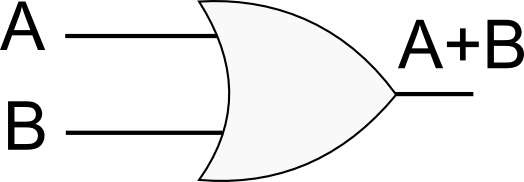
\includegraphics[height = 1in, width = 2in]{or.png}
   \end{column}\pause
   \begin{column}{5cm}
    \begin{tabular}{|c|c|c|}
     \hline
     A & B & A + B \\
     \hline	
     0 & 0 & 0 \\
     0 & 1 & 1 \\
     1 & 0 & 1 \\
     1 & 1 & 1 \\ 
     \hline
    \end{tabular}
   \end{column}

  \end{columns}
\end{center}
\end{frame}

\begin{frame}
  \frametitle{Básico - Portas lógicas}
\begin{center}
   \textbf{\huge{Porta AND}}
   \begin{columns}[c]
   \begin{column}{5cm}
    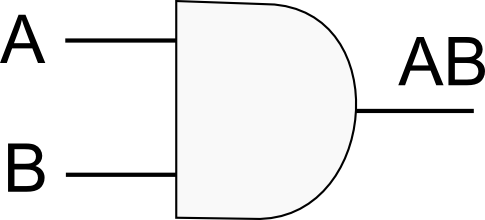
\includegraphics[height = 1in, width = 2in]{and.png}
   \end{column}\pause
   \begin{column}{5cm}
    \begin{tabular}{|c|c|c|}
     \hline
     A & B & AB \\
     \hline	
     0 & 0 & 0 \\
     0 & 1 & 0 \\
     1 & 0 & 0 \\
     1 & 1 & 1 \\ 
     \hline
    \end{tabular}
   \end{column}

  \end{columns}
\end{center}
\end{frame}

\begin{frame}
  \frametitle{Básico - Portas lógicas}
  \begin{center}
    \textbf{\huge{Porta Inversora}}
    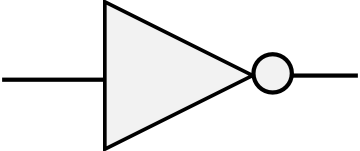
\includegraphics[height = 1in, width = 2in]{inversora.png}
  \end{center}
\end{frame}

\begin{frame}
  \frametitle{Básico - Portas lógicas}
\begin{center}
   \textbf{\huge{Porta NOR}} 
   \begin{columns}[c]
   \begin{column}{5cm}
    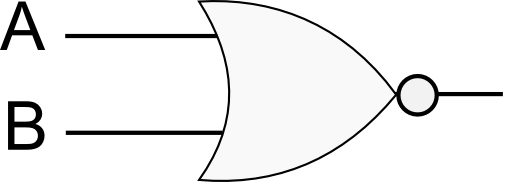
\includegraphics[height = 1in, width = 2in]{nor.png}
   \end{column}\pause
   \begin{column}{5cm}
    \begin{tabular}{|c|c|c|}
     \hline
     A & B & $\overline{A + B}$ \\
     \hline	
     0 & 0 & 1 \\
     0 & 1 & 0 \\
     1 & 0 & 0 \\
     1 & 1 & 0 \\ 
     \hline
    \end{tabular}
   \end{column}

  \end{columns}
\end{center}
\end{frame}

\begin{frame}
  \frametitle{Básico - Portas lógicas}
\begin{center}
   \textbf{\huge{Porta NAND}} 
   \begin{columns}[c]
   \begin{column}{5cm}
    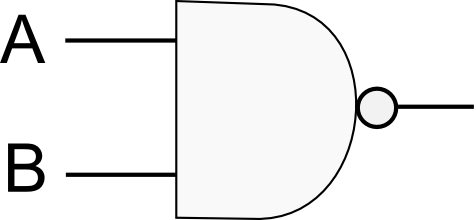
\includegraphics[height = 1in, width = 2in]{nand.png}
   \end{column}\pause
   \begin{column}{5cm}
    \begin{tabular}{|c|c|c|}
     \hline
     A & B & $\overline{AB}$ \\
     \hline	
     0 & 0 & 1 \\
     0 & 1 & 1 \\
     1 & 0 & 1 \\
     1 & 1 & 0 \\ 
     \hline
    \end{tabular}
   \end{column}

  \end{columns}
\end{center}
\end{frame}

\begin{frame}
  \frametitle{Básico - Portas lógicas}
\begin{center}
   \textbf{\huge{Porta XOR}} 
   \begin{columns}[c]
   \begin{column}{5cm}
    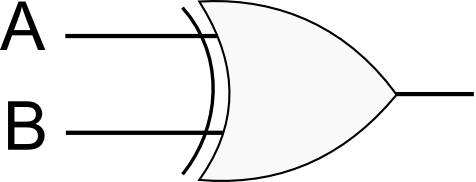
\includegraphics[height = 1in, width = 2in]{xor.png}
   \end{column}\pause
   \begin{column}{5cm}
    \begin{tabular}{|c|c|c|}
     \hline
     A & B & $A \oplus B$ \\
     \hline	
     0 & 0 & 0 \\
     0 & 1 & 1 \\
     1 & 0 & 1 \\
     1 & 1 & 0 \\ 
     \hline
    \end{tabular}
   \end{column}

  \end{columns}
\end{center}
\end{frame}

\begin{frame}
  \frametitle{Básico - Portas lógicas}
\begin{center}
   \textbf{\huge{Porta XNOR}}
   \begin{columns}[c]
   \begin{column}{5cm}
    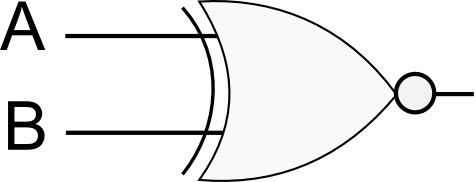
\includegraphics[height = 1in, width = 2in]{xnor.png}
   \end{column}\pause
   \begin{column}{5cm}
    \begin{tabular}{|c|c|c|}
     \hline
     A & B & $\overline{A \oplus B}$ \\
     \hline	
     0 & 0 & 1 \\
     0 & 1 & 0 \\
     1 & 0 & 0 \\
     1 & 1 & 1 \\ 
     \hline
    \end{tabular}
   \end{column}

  \end{columns}
\end{center}
\end{frame}

\begin{frame}
  \frametitle{Básico - Operações booleanas}
\begin{columns}[c]
  \begin{column}{3cm}
   \begin{itemize}
   \item $x.0 = 0 $  \pause
   \item $x.1 = x $  \pause 
   \item $x.x = x $  \pause
   \item $x.\overline{x} = 0 $  \pause
   \item $x + 0 = x $  \pause
   \item $x + 1 = 1 $  \pause 
   \item $x + x = x $  \pause 
   \item $x + \overline{x} = 0 $  \pause 
   \item $x + y = y + x $  \pause 
  \end{itemize}
 \end{column} 
  
  \begin{column}{7cm}
   \begin{itemize}
   \item $x.y = y.x $  \pause
   \item $x + (y + z) = (x + y) + z = x + y + z $  \pause 
   \item $x(yz) = (xy)z = xyz $  \pause
   \item $x(y + z) = xy + xz $  \pause
   \item $(w + x)(y + z) = wy + xy + wz + xz$  \pause
   \item $x + xy = x $  \pause 
   \item $x + \overline{x}y = x + y $  \pause 
   \item $\overline{x} + xy = \overline{x} + y$  \pause 
   \item $\overline{(x + y)} = \overline{x}\overline{y} $  \pause 
   \item $\overline{(xy)} = \overline{x} + \overline{y} $   
  \end{itemize}
  \end{column}
\end{columns}
\end{frame}



  
%SLIDES == CIRCUITOS
\section{Circuitos}
\begin{frame}
  \frametitle{Circuitos}
  \begin{itemize}
   \item A eletrônica digital possui dezenas de componentes, o conhecimento do comportamento destes é fundamental para a elaboração de projetos na área. 
	 Todos os componentes aqui apresentados costumas ser utilizados em algumas das principais etapas de projetos de microcontroladores. Vale observar 
	 que estes componentes podem ser feitos em VHDL e combinados.
  \end{itemize}
\end{frame}

%SLIDES == REGISTRADORES
\section{Registradores}
\begin{frame}
  \frametitle{Registradores}
  \begin{enumerate}
   \item Imagine que se um circuito deva receber de forma serial o seguinte dados: 10011101. A opção mais obvia seria a utilização de Flip-Flops, onde 
	 teríamos um Flip-Flop para cada bit. \pause
   \item Com base na ideia citada acima podemos especificar um registrador da seguinte forma: \pause  
    \begin{block}{\textbf{Especificação}}
     Um registrador é um circuito contendo dois ou mais Flip-Flops conectados juntos, de forma que todos eles trabalhem da mesma forma e são 
	    sincronizados pelo mesmo sinal de clock.
    \end{block} \pause
 
   \item Flip-Flops podem possuir algumas entradas síncronas, tal como o “Clear” (também conhecido por “Reset”) e “Enable”. Estas entradas são extremamente 
	   uteis quando se deseja combinar vários componentes.
  \end{enumerate}
\end{frame}

\begin{frame}
  \frametitle{Registradores}
  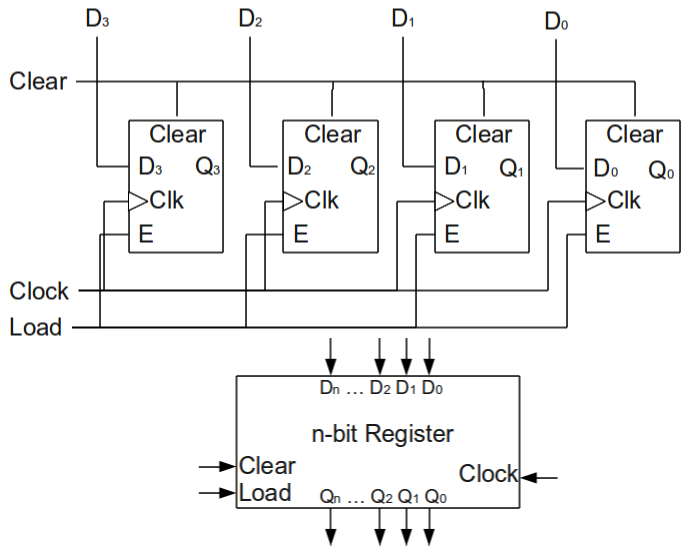
\includegraphics[height=2in, width = 3in]{registrador_padrao.png}
\end{frame}

%SLIDES == REGISTRADOR DE DESLOCAMENTO
\begin{frame}
  \frametitle{Registrador de deslocamento (Shift Register)}
  \begin{enumerate}
   \item Um registrador de deslocamento é muito semelhante a um registrador convencional, diferenciado-se na forma como os dados são inseridos, segue uma 
	 pequena descrição formal:\pause
    \begin{block}{\textbf{Especificação}}
      Um registrador de deslocamento é um grupo de Flip-Flops organizados de modo que o número binário armazenado nos Flip-Flops sejam deslocados de 
	     um Flip-Flop para o seguinte a cada pulso de clock. 
    \end{block} \pause
  
    \item Um dos principais uso do registrador de deslocamento é para conversão de entradas de dado serial para um dado paralelo ou vice-versa.
  \end{enumerate}
\end{frame}

\begin{frame}
  \frametitle{Registrador de deslocamento (Shift Register)}
  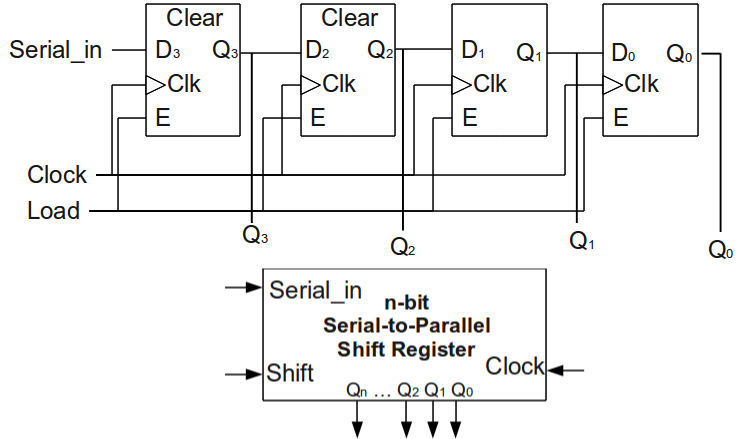
\includegraphics[height=2in, width = 3in]{registrador_de_deslocamento.png}
\end{frame}

%SLIDES == MESCLANDO CARACTERISTICAS
\begin{frame}
 \frametitle{Mesclando características}
  \begin{enumerate}
    \item Com base nos dois tipos de registradores apresentados podemos mesclar as características de ambos em um único circuito. O novo componente terá as 
	 seguintes características:\pause
    \begin{enumerate}
      \item Poderá receber uma entrada paralela e serial. Sendo que esta opção é selecionada por meio de uma entrada assíncrona chamada “Enable”.\pause
      \item O dado inserido poderá ser deslocado para a esquerda ou para a direita.\pause
      \item O registrador poderá apresentar uma saída serial ou paralela. 
    \end{enumerate}
  \end{enumerate}
\end{frame}

\begin{frame}
  \frametitle{Mesclando características}
  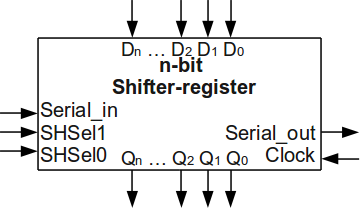
\includegraphics[height=2in, width = 3in]{registrador_deslocamentoLR_entrada_paralela.png}
\end{frame}

%SLIDES == CONTADORES BINÁRIOS
\section{Contadores}
\begin{frame}
 \frametitle{Contadores binários}
  \begin{enumerate}
   \item Existem diversas variações de contadores, que podem seguir diversas sequências especificas (decimal, BCD, binária, etc). Contudo atentamos nos 
	 contadores binários sequenciais que possuem carry (também conhecido por “vai um”).\pause
   \item Ao se combinar vários meio somadores e ligá-los a Flip-Flops cria-se os chamados somadores.
  \end{enumerate}
\end{frame}

\begin{frame}
  \frametitle{Contador binário}
  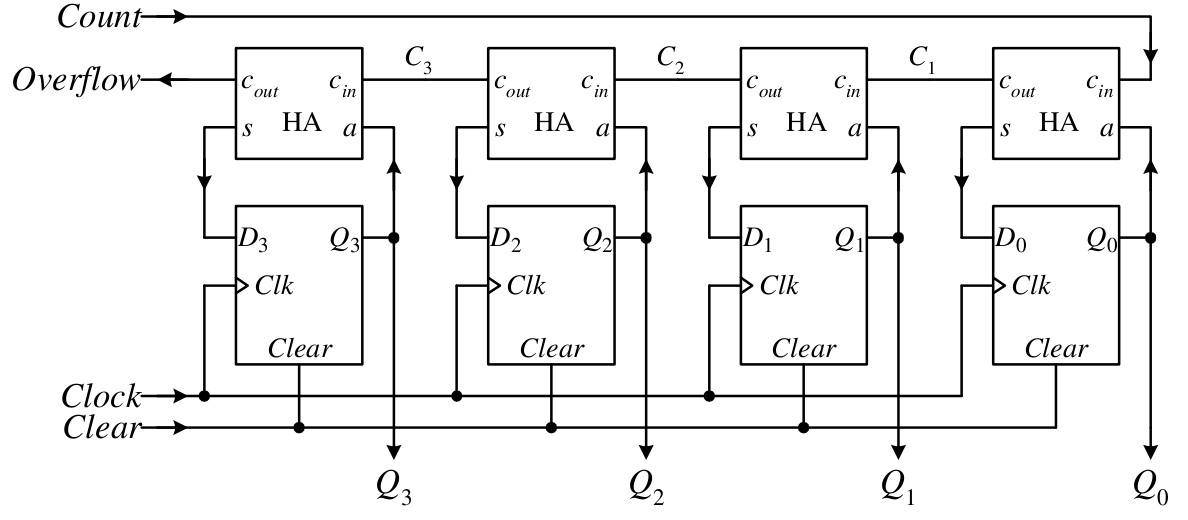
\includegraphics[height=2in, width=4in]{contador.png}
\end{frame}

\begin{frame}
 \frametitle{Contador binário}
 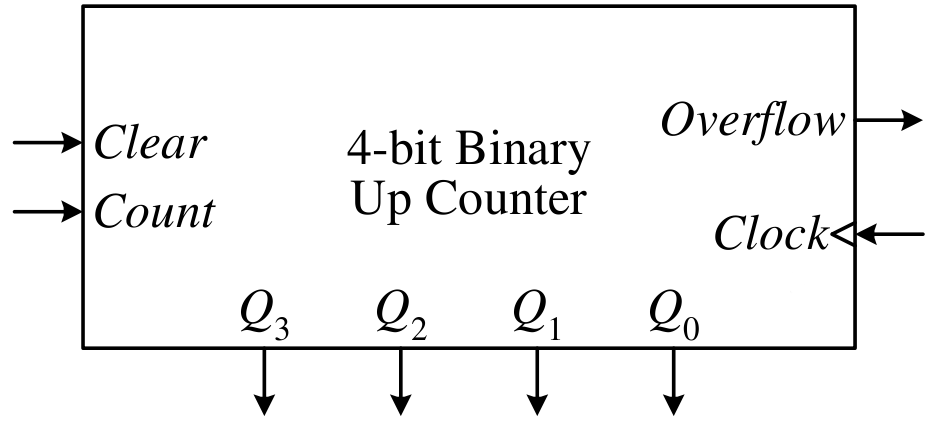
\includegraphics[height=2in, width=4in]{contador_simbolo.png}
\end{frame}

%CONTADOR BINÁRIO CRESCENTE - DECRESCENTE
\begin{frame}
  \frametitle{Contador binário crescente – decrescente (Up-down Counter)}
\begin{enumerate}
  \item Trata-se de um contador binário que conta em ordem crescente ou decrescente de acordo com um sinal. \pause
  \item \textbf{Geralmente} adiciona-se uma entrada chamada “Down” que quando recebe um sinal “1” realiza a contagem de forma decrescente.
 \end{enumerate}
\end{frame}

\begin{frame}
 \frametitle{Contador binário crescente – decrescente (Up-down Counter)}
  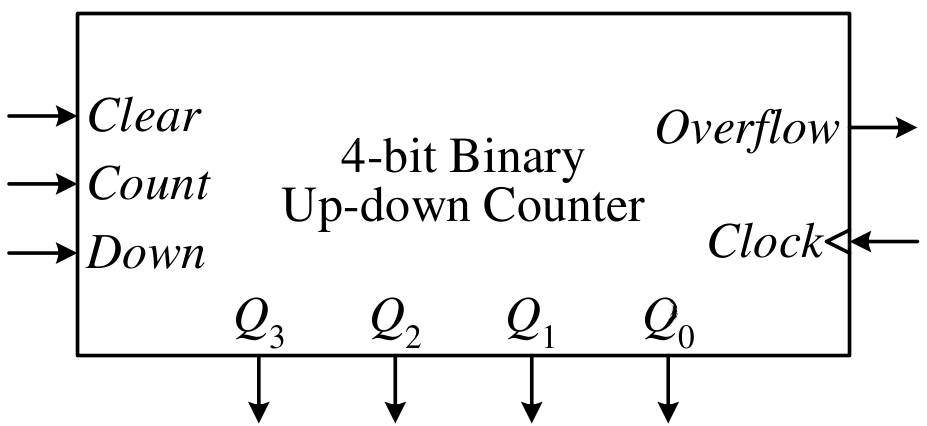
\includegraphics[height=2in, width=4in]{contador_crescente_decrescente.png}
\end{frame}

%SLIDE == CONTADOR BINÁRIO CRESCENTE-DECRESCENTE COM CARREGAMENTO PARELELO
\begin{frame}
  \frametitle{Contador binário crescente-decrescente com carregamento paralelo}
 \begin{enumerate}
  \item Possui o funcionamento muito parecido com o contador citado em 5.1, com a diferença que este recebe um valor inicial de entrada que 
	servirá de base para a contagem crescente ou decrescente.\pause
  \item Uma entrada “load” é adicionada para indicar se um valor deve ser carregado ou não para o contador.
 \end{enumerate}
\end{frame}

\begin{frame}
 \frametitle{Contador binário crescente-decrescente com carregamento paralelo}
  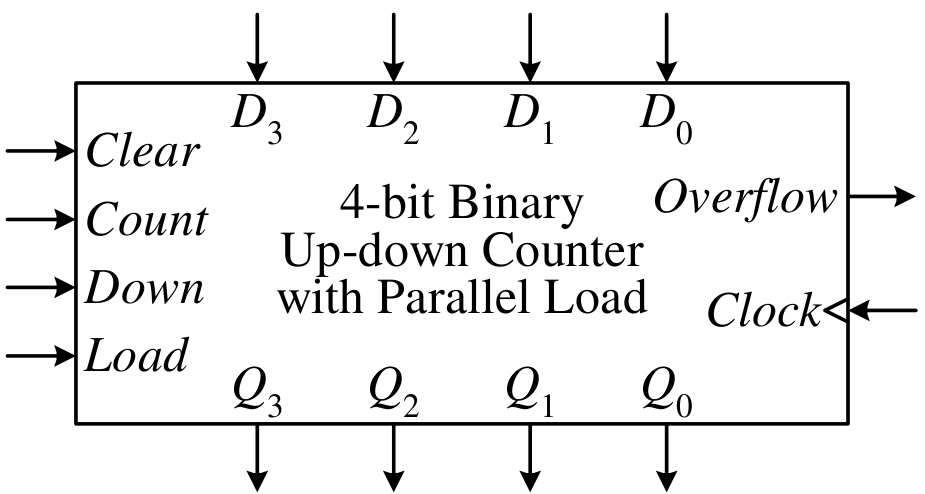
\includegraphics[height=2in, width=4in]{contador_crescente_decrescente_com_entrada_paralela.png}
\end{frame}

%SLIDE == REGISTER FILES
\section{Register files}
\begin{frame}
 \frametitle{Register files}
\begin{enumerate}
  \item Sabe-se que um registrador pode armazenar dados, contudo se quisermos armazenar uma quantidade maior de dados torna-se mais interessante 
	tratar estes registradores como unidades. \pause
  \item Ao invés de termos uma série de registradores individuais, nos podemos ter um vetor de registradores. Este vetor de registrador também é 
	conhecido por Register file.\pause
  \item Em um Register files, todos os respectivos sinais de controle para um registrador individual são conectados em comum. Além disto, toda 
	entrada de dados e linha de saída para todos os registradores são também conectados em comum. \pause
  \item Register files tem somente uma linha de entrada e também possui linhas de endereço que são utilizadas para especificar que registrador em 
	um register file deve ser acessado. 
 \end{enumerate}
\end{frame}

\begin{frame}
 \frametitle{Register files}
 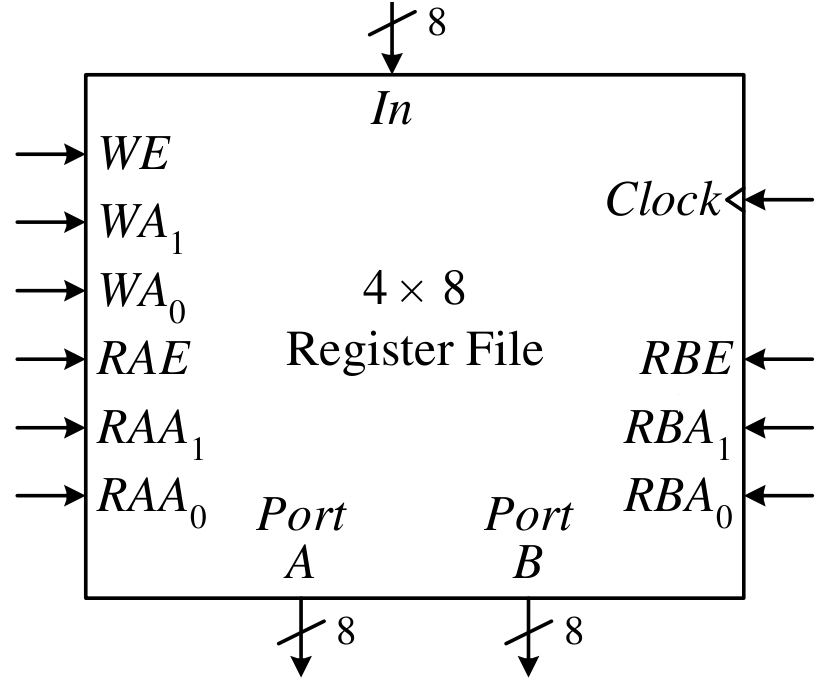
\includegraphics[height=2in, width=3.5in]{register_files.png}
\end{frame}

\begin{frame}
 \frametitle{Register files}
 \begin{enumerate}
  \item Register files é um tipo de memória extremamente veloz devido aos seguintes motivos: \pause
    \begin{enumerate}
      \item É composto por registradores.\pause
      \item Possui uma entrada paralela dedicada \pause
      \item Possui uma saída paralela dedicada \pause
      \item Possui linhas de entrada dedicadas a especificar o registrador algo das operações
    \end{enumerate}
 \end{enumerate}
\end{frame}

%SLIDE == RAM
\section{RAM}
\begin{frame}
 \frametitle{Static Random Access Memory (RAM)}
 \begin{enumerate}
  \item Memórias RAM são semelhantes aos Register files, contudo estas possuem mais locais para armazenar dados. 
	Contudo o aumento no tamanho de armazenamento tem seus impactos, que são: \pause
    \begin{enumerate}
      \item Muitas vezes queremos muita memória e queremos que o circuito seja o menor possível, então precisamos fazer cada célula menor possível.\pause
      \item Precisamos usar um caminho de dados comum para leitura e escrita de dados na memória. \pause
    \end{enumerate}
  \item Temos em memórias RAM linhas de endereçamento para acesso da memória e uma linha responsável pelos dados que chamamos de A (A vem de Adress) 
	e Di (D vem de data).
 \end{enumerate}
\end{frame}

\begin{frame}
 \frametitle{Static Random Access Memory (RAM)}
  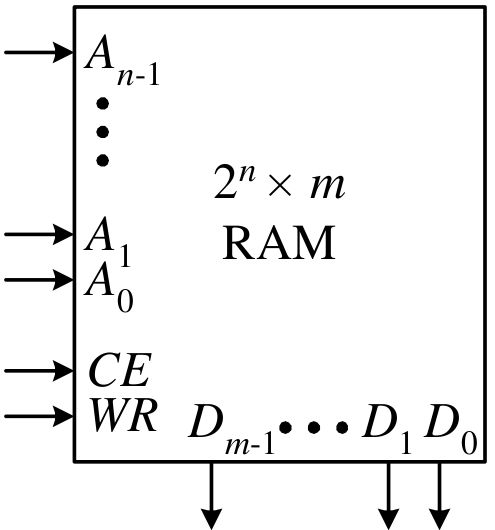
\includegraphics[height=2in, width=3in]{RAM.png}
\end{frame}

%SLIDE == REFERENCIA BIBLIOGRAFICA
\section{Bibliografia}
\begin{frame}
 \frametitle{Referências bibliográficas}
 \begin{enumerate}
  \item Digital Logic and Microprocessor Design With VHDL – Enoch O . Hwang
  \item Sistemas digitais princípios e aplicação - Tocci
 \end{enumerate}
\end{frame}

\end{document}
